\section{Tournament Manager Software}\label{secTournamentManagerSoftware}

All three StarCraft AI competitions covered in this paper use the same open-source tool, with varying number of modifications, to automate the bot games. The tool is called StarCraft AI Tournament Manager (TM) \footnote{\url{http://github.com/davechurchill/StarcraftAITournamentManager}} and was created / maintained by David Churchill and Richard Kelly for the AIIDE competition. It allows tournaments of thousands of one-on-one games to be played automatically. The original version of the software was created in 2011 for the AIIDE StarCraft AI Competition. The CIG StarCraft AI Competition has used the TM software since 2012, and SCCAIT has used a modified version of the tournament manager since 2014. 

The TM software supports both round robin and one vs. all tournaments for testing one bot against others. The server stores all bot and map files, as well as results and replay files generated by the BroodWar clients. Files are sent over Java sockets between the server and client machines. The tournament manager supports bots using different versions of BWAPI, and support for new versions can easily be added, allowing bots written in any version of BWAPI to play in the same tournament. Each client machine currently requires an installation of StarCraft: BroodWar version 1.16.1.

\begin{figure}[t]
  \centering
  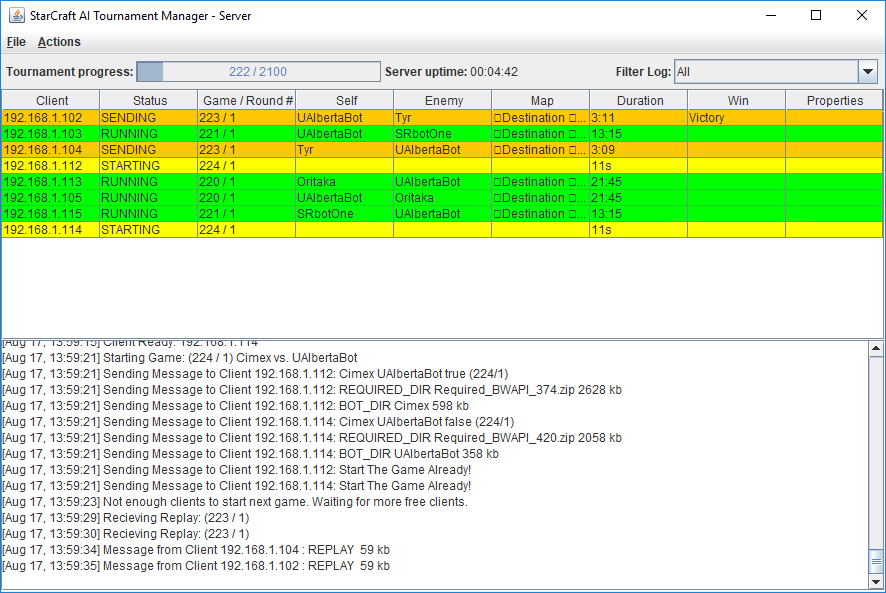
\includegraphics[width=1\columnwidth]{fig/tournament-manager-screenshot.png}
  \caption{Tournament Manager server GUI}
  \label{tmServerGUI}
\end{figure}

The TM software uses a server-client architecture distributed over multiple physical or virtual machines connected via LAN, with one machine acting as a server (coordinating the matchups and processing results) and any number of other machines acting as clients (running the bots and StarCraft). The tournament manager is written entirely in Java. The clients should run on Windows machines due to system requirements of StarCraft, while the server is fully platform-independent. All the data sent and received is compressed and passed through Java sockets over TCP/IP, so no special network configuration is required.

\subsection{Server}

When running the software, one machine acts as a server for the tournament. The server machine holds central repository of all the bot files, their custom I/O data files, cumulative results, and replay files. The server monitors and controls each client remotely and displays the tournament's progress in real time via the server GUI (see Figure~\ref{tmServerGUI}), also writing the current results to an HTML file every few seconds.

%\begin{figure}[t]
%  \centering
%  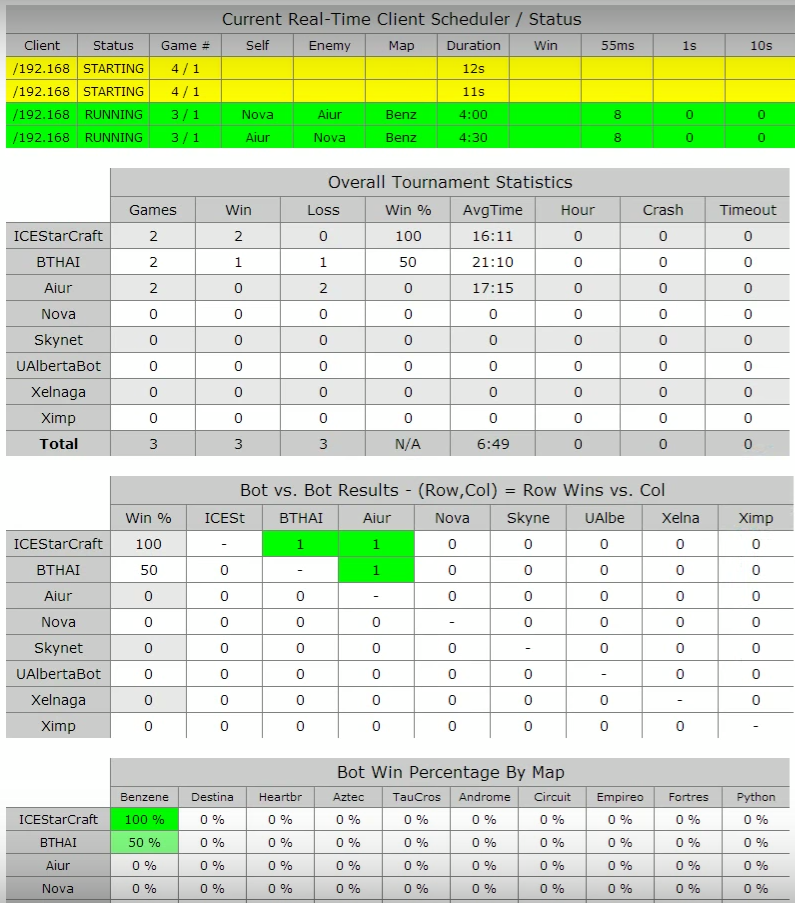
\includegraphics[width=1\columnwidth]{fig/tournament-manager-screenshot2.png}
%  \caption{Tournament Manager results in HTML format}
%  \label{tmServerHTML}
%\end{figure}

The server program has a threaded component which monitors client connections and detects disconnections, maintaining a current list of clients. Each client is in one of the following states at all times (column ``Status'' in Figure~\ref{tmServerGUI}):

\begin{itemize}
\item READY: Client is ready to start a game of StarCraft.
\item STARTING: Client has started the StarCraft LAN lobby but the match has not yet begun.
\item RUNNING: A game of StarCraft is currently in progress on the client machine.
\item SENDING: Client has finished the game and is sending results and data back to the server.
\end{itemize}

The server's main scheduling loop tries to schedule the next game from the games list every 2 seconds. A new game is started whenever both of these conditions are true:

\begin{enumerate}
\item two or more Clients are in READY state, and
\item no clients are in STARTING state.
\end{enumerate}

\noindent Once these two conditions are met, the server sends the required bot files, BWAPI version used by the bots, map file, and DLL injector to the client machines. The state of those clients is then set to STARTING.

Each client is handled by a separate thread in the server, and if the client is STARTING, RUNNING, or SENDING, it sends periodic status updates back to the server once per second for remote monitoring. Data updates include current game time, time-out information, map name, game ID, etc. When a client finishes a game, it also sends the results, I/O data files created by the bots and replay files, which are all stored on the server. This process is repeated until the tournament has finished.

Shutting down the server via the GUI will cause all the client games to stop and all clients to shut down and properly clean up remote machines. The tournament can be resumed upon re-launching the server as long as the results file, games list, and settings files do not change. If the server is shut down with games in progress (results not yet received by the server), those games will be rescheduled and played again. The server GUI can send commands to the client machines, take screenshots of the client machine desktops, and remove clients from the tournament. Individual client machines can be added to and removed without stopping the current tournament.

\subsection{Client}

The client software can be run on as many machines as needed. After an initial setup of the client machine (installing StarCraft, required libraries, etc.) the client software connects to the server machine via TCP/IP and awaits instructions.

The client machine will stay idle until it receives instructions from the server that a game should be run. Once the client receives the instructions and required files from the server, it ensures that no current StarCraft processes are running, ensures a clean working StarCraft directory, records a current list of the running processes on the client machine, writes the BWAPI settings file, and starts the game. When the game starts, a custom BWAPI Tournament Module DLL is injected to StarCraft process. It updates a special GameState file on the hard drive every few frames -- this is used to monitor the current state of the running StarCraft game. The client software watches this file to check for various conditions, such as bot time-outs, crashes, game frame progression, and game termination. While the game is running, the client also sends the contents of the GameState file to the server once per second for centralized monitoring.

Once the game has ended or was terminated for any reason, the results of the game, replay files, and bot's I/O data files are sent to the server. After this, the client shuts down any processes on the machine which were not running when the game began, to prevent crashed proxy bots or stray threads from hogging system resources from future games. StarCraft is shut down, the machine is cleaned of any files written during the previous game, and the client state is reverted to READY.

Since 2017, client machines can be labeled with custom properties such as “extra ram” or “GPU”, and bots can be labeled with matching custom requirements. Only clients that have all the requirements of a bot will be used for hosting that bot, and clients with special properties will be reserved to be used last to increase their availability for bots requiring them. The TM software also supports both DLL based bots and bots with their own executable file which interface with BWAPI. This server-client architecture has allowed tens of thousands of games to play played in AI competitions each year.
